\part{Implementation}

\chapter{Backend, Database, and IoT Data Ingestion}

\section{Introduction}

This chapter describes the implementation of the backend, database, and IoT ingestion pipeline. It explains how MQTT messages become database records, Digital Twin states, ML predictions, and dashboard updates.

\section{FastAPI backend organization}

The backend is implemented with FastAPI. It exposes REST endpoints under the /api/v1 prefix, provides automatic OpenAPI documentation, configures CORS for frontend/mobile access, initializes services, and starts the MQTT subscriber when the system is configured for MQTT data source mode.

\section{API modules}

The API is organized around users, farms, plots, soil profiles, crops, zones, sensors, weather records, irrigation events, Digital Twins, predictions, recommendations, control commands, simulations, dashboard aggregation, device control, ML proxy, forecasting, system status, and debugging. This organization reflects the functional separation of the platform.

\section{MQTT payload structure}

Sensor messages are published on sensors/data as JSON. A typical message contains device\_id, timestamp, soil\_moisture, soil\_temperature, temperature, humidity, pressure, leaf\_wetness, light\_intensity, rainfall\_current, rainfall\_hour, rainfall\_day, wind\_direction, and wind\_speed. WeMos status messages contain device\_id and digital pin states such as D5 and D3.

\begin{figure}[H]
    \centering
    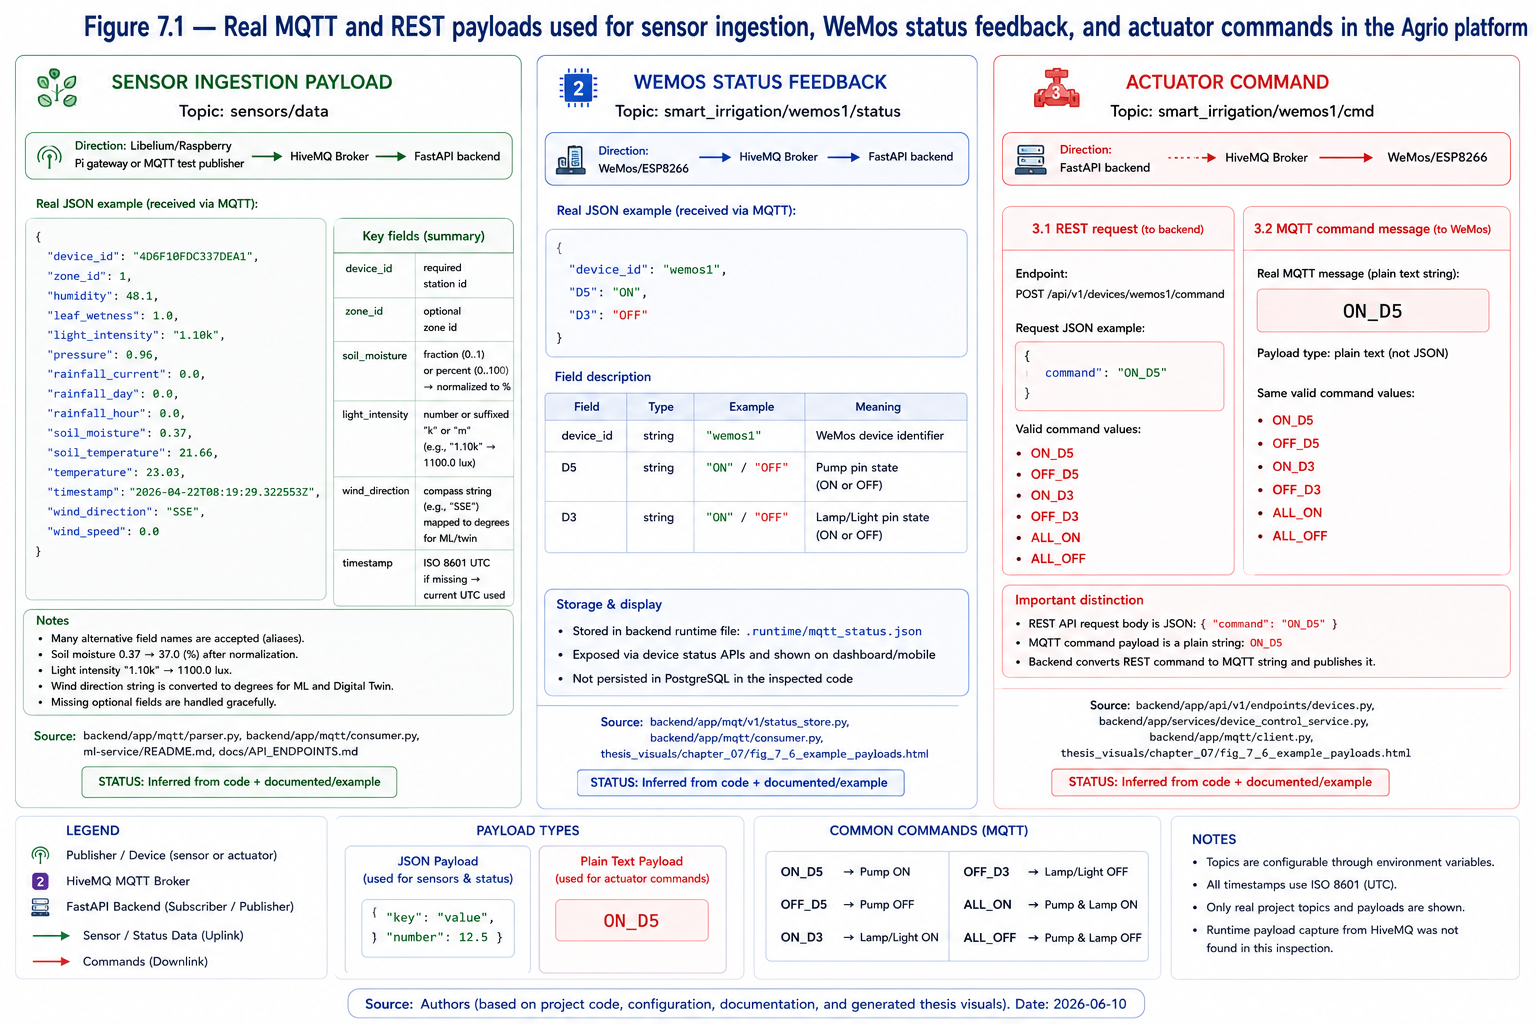
\includegraphics[width=0.9\textwidth,height=0.75\textheight,keepaspectratio]{figures/chapter_07/Figure 7.1 — Example MQTT payloads used for sensor ingestion, WeMos status feedback, and actuator commands.png}
    \caption{Example MQTT payloads used for sensor ingestion, WeMos status feedback, and actuator commands. Source: Authors.}
    \label{fig:7-6-example-mqtt-payloads-used-for-sensor-ingestion-wemos-status-feedb}
\end{figure}

\section{Parser and normalization}

The parser validates JSON, accepts aliases, converts soil moisture fractions into percentages, parses timestamps, normalizes numeric values, handles light-intensity suffixes, and normalizes wind direction. This step is essential because IoT messages can be inconsistent and sensor formats may differ.

\section{Device mapping and persistence}

After parsing, the backend resolves the device and management zone. It creates sensor mappings if required, stores sensor\_readings, stores weather\_records when environment fields exist, and updates the runtime MQTT status store. The source field preserves the origin of the record, for example mqtt:device\_id.

\section{Real-time pipeline}

The real-time pipeline evaluates sensor health, updates zone state, calls the ML service, stores prediction results, appends zone\_state\_history, and generates recommendations. This pipeline converts raw measurements into actionable Digital Twin data.

\section{PostgreSQL schema}

The PostgreSQL schema contains tables for users, farms, plots, zones, soil profiles, crops, irrigation networks, sensors, readings, weather records, device health, forecasts, digital twins, zone states, predictions, simulations, recommendations, alerts, commands, events, and feedback. This structure supports traceability from sensor data to action.

\begin{figure}[H]
    \centering
    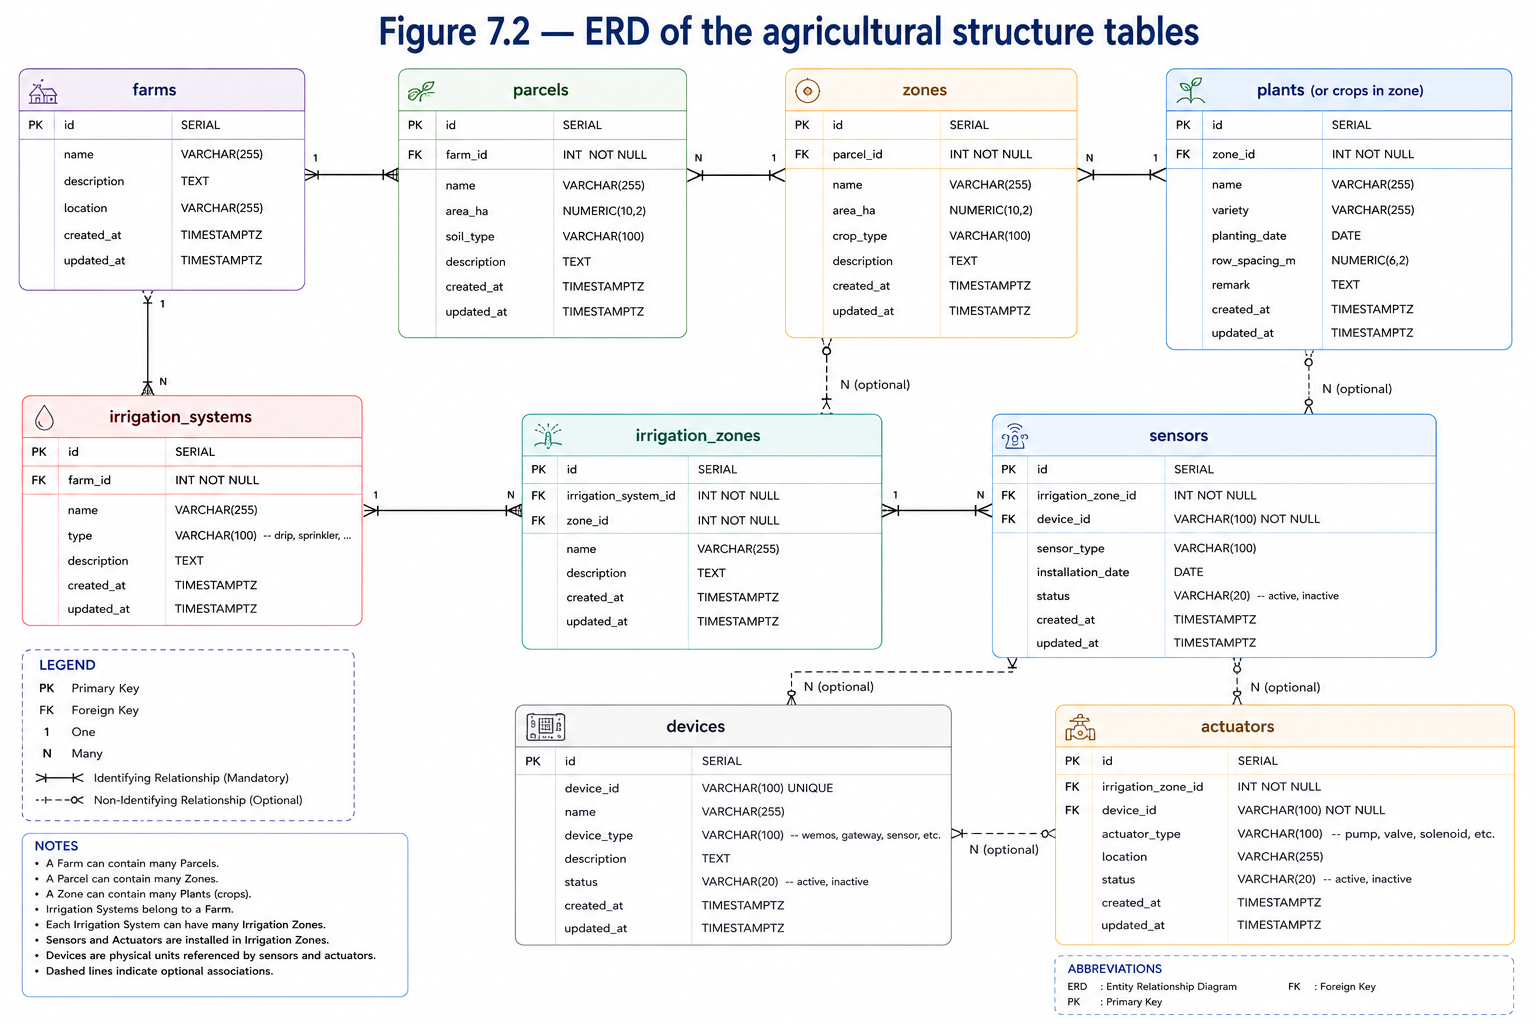
\includegraphics[width=0.9\textwidth,height=0.75\textheight,keepaspectratio]{figures/chapter_07/Figure 7.2 — ERD of the agricultural structure tables.png}
    \caption{ERD of the agricultural structure tables. Source: Authors.}
    \label{fig:7-5a-erd-of-the-agricultural-structure-tables}
\end{figure}

\begin{figure}[H]
    \centering
    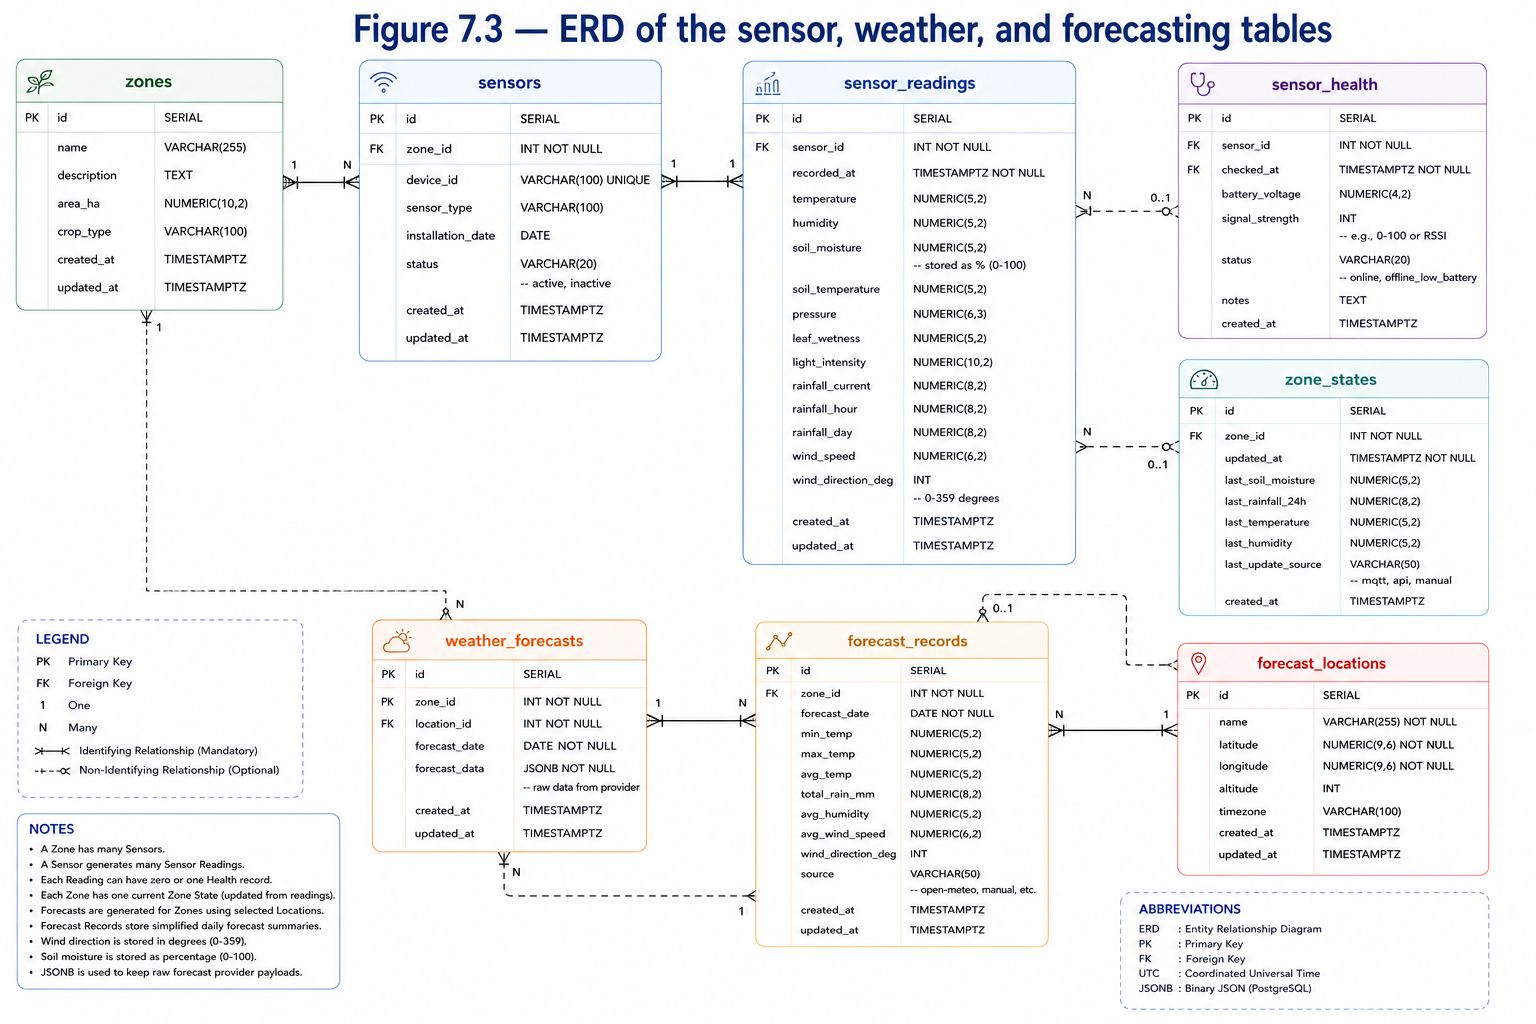
\includegraphics[width=0.9\textwidth,height=0.75\textheight,keepaspectratio]{figures/chapter_07/Figure 7.3 — ERD of the sensor, weather, and forecasting tables.png}
    \caption{ERD of the sensor, weather, and forecasting tables. Source: Authors.}
    \label{fig:7-5b-erd-of-the-sensor-weather-and-forecasting-tables}
\end{figure}

\begin{figure}[H]
    \centering
    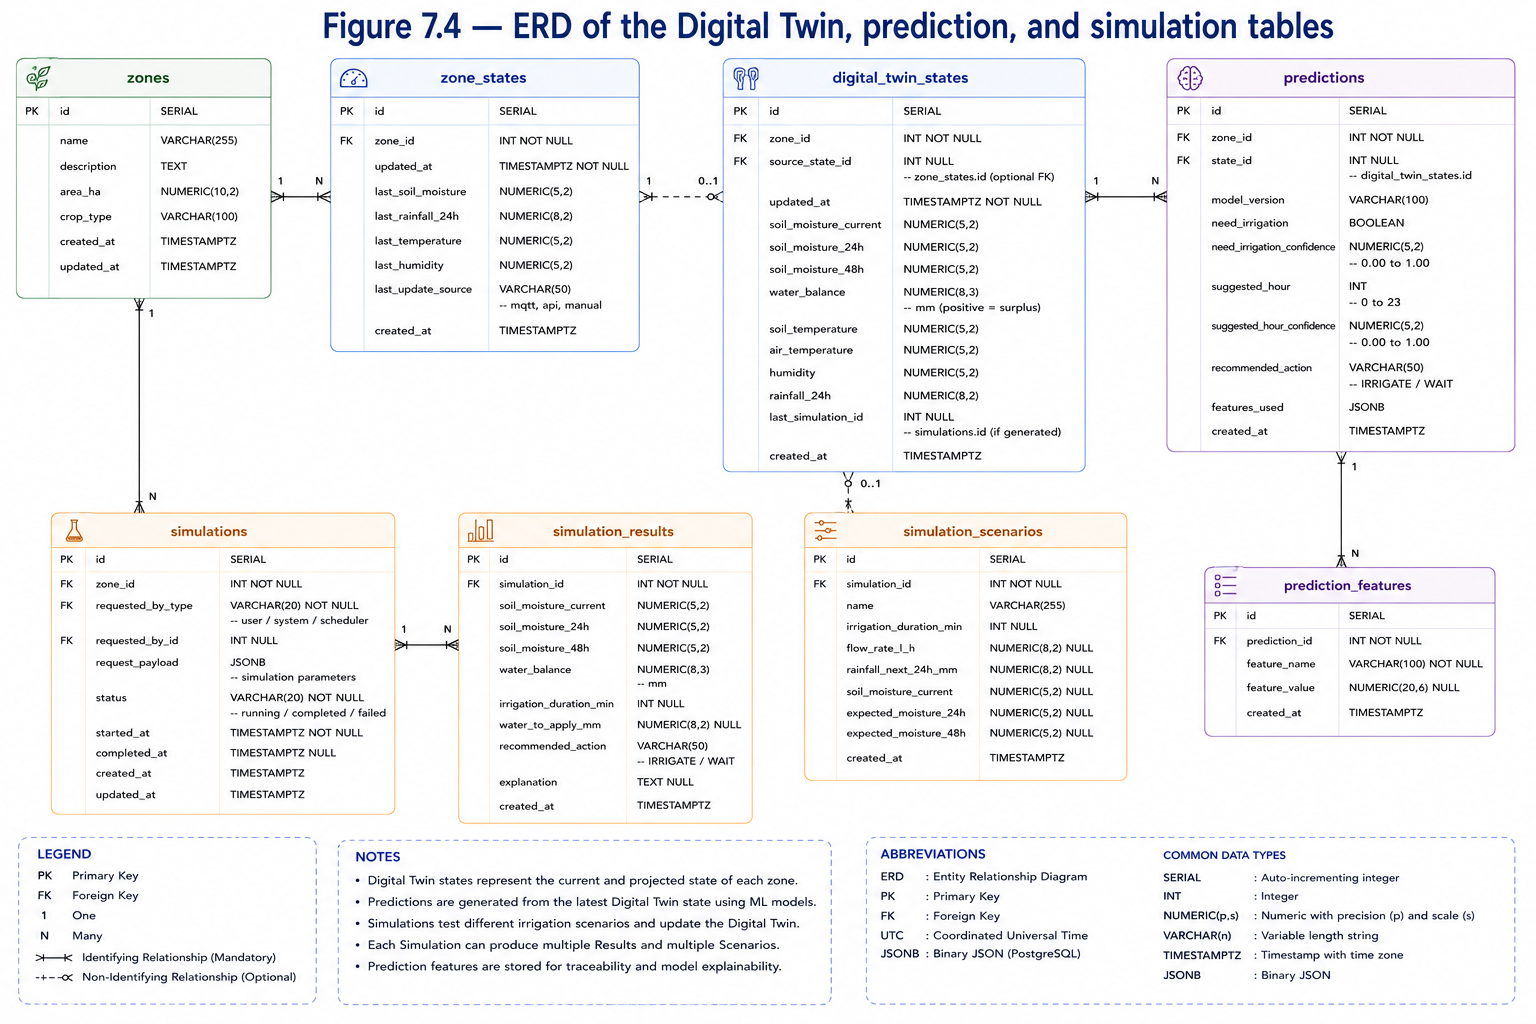
\includegraphics[width=0.9\textwidth,height=0.75\textheight,keepaspectratio]{figures/chapter_07/Figure 7.4 — ERD of the Digital Twin, prediction, and simulation tables.png}
    \caption{ERD of the Digital Twin, prediction, and simulation tables. Source: Authors.}
    \label{fig:7-5c-erd-of-the-digital-twin-prediction-and-simulation-tables}
\end{figure}

\begin{figure}[H]
    \centering
    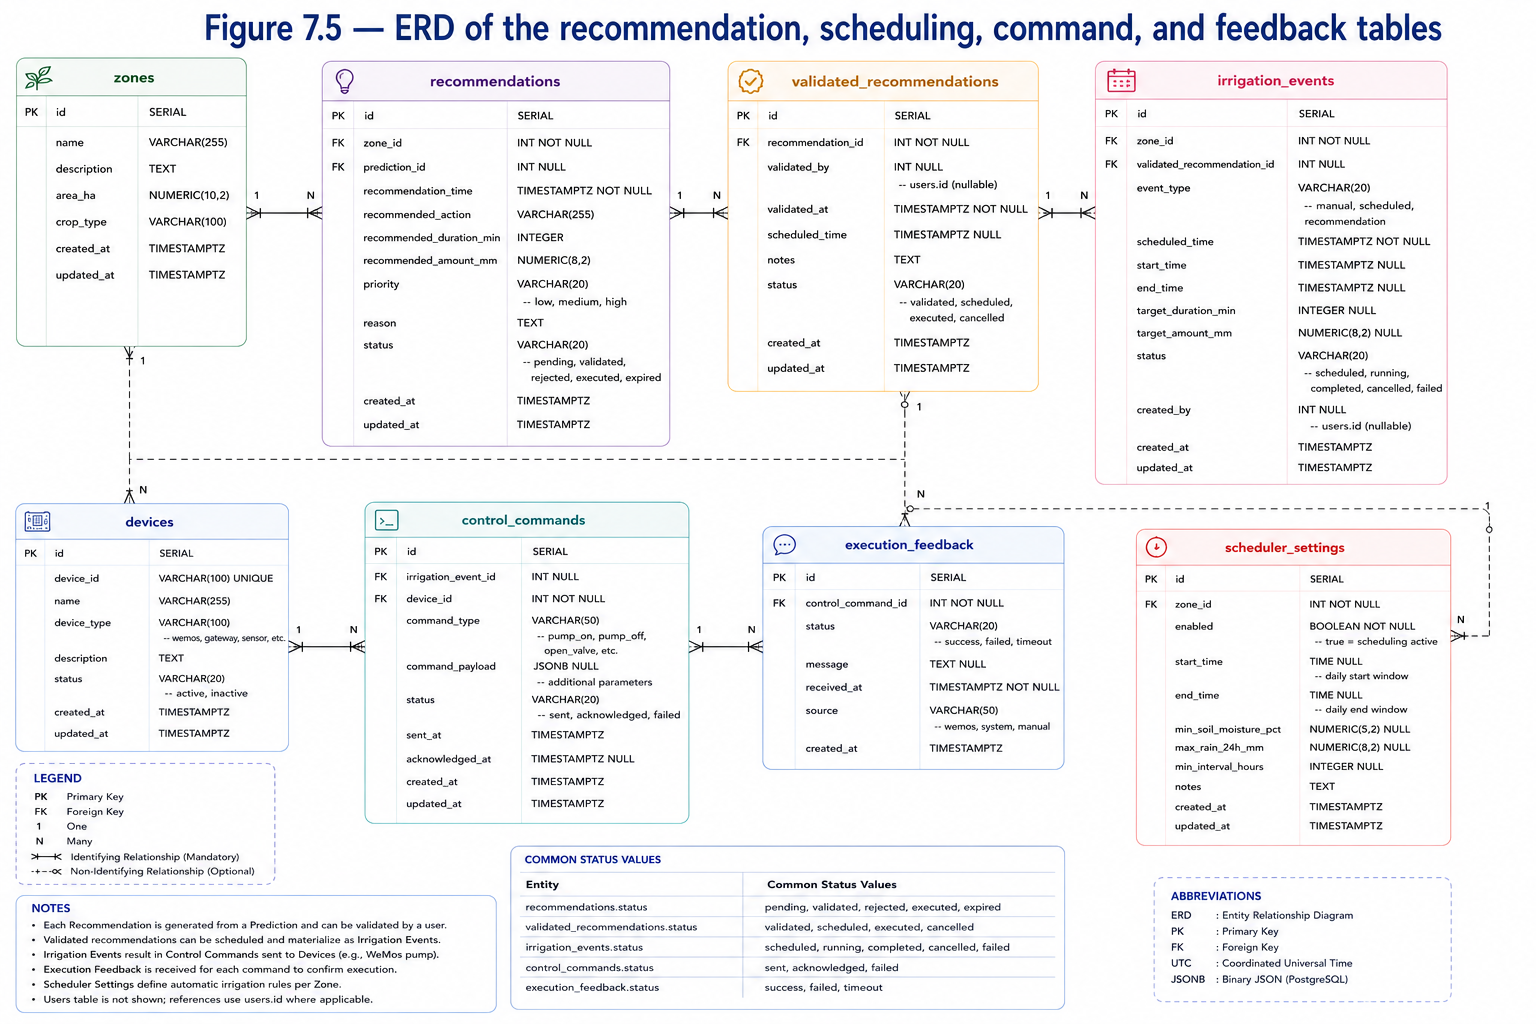
\includegraphics[width=0.9\textwidth,height=0.75\textheight,keepaspectratio]{figures/chapter_07/Figure 7.5 — ERD of the recommendation, scheduling, command, and feedback tables.png}
    \caption{ERD of the recommendation, scheduling, command, and feedback tables. Source: Authors.}
    \label{fig:7-5d-erd-of-the-recommendation-scheduling-command-and-feedback-tables}
\end{figure}

\section{Runtime sequence}

The runtime sequence demonstrates how a sensor message travels from the sensor station to the MQTT broker, backend subscriber, parser, database, real-time pipeline, ML service, dashboard, device-control service, WeMos, and status feedback.

\begin{figure}[H]
    \centering
    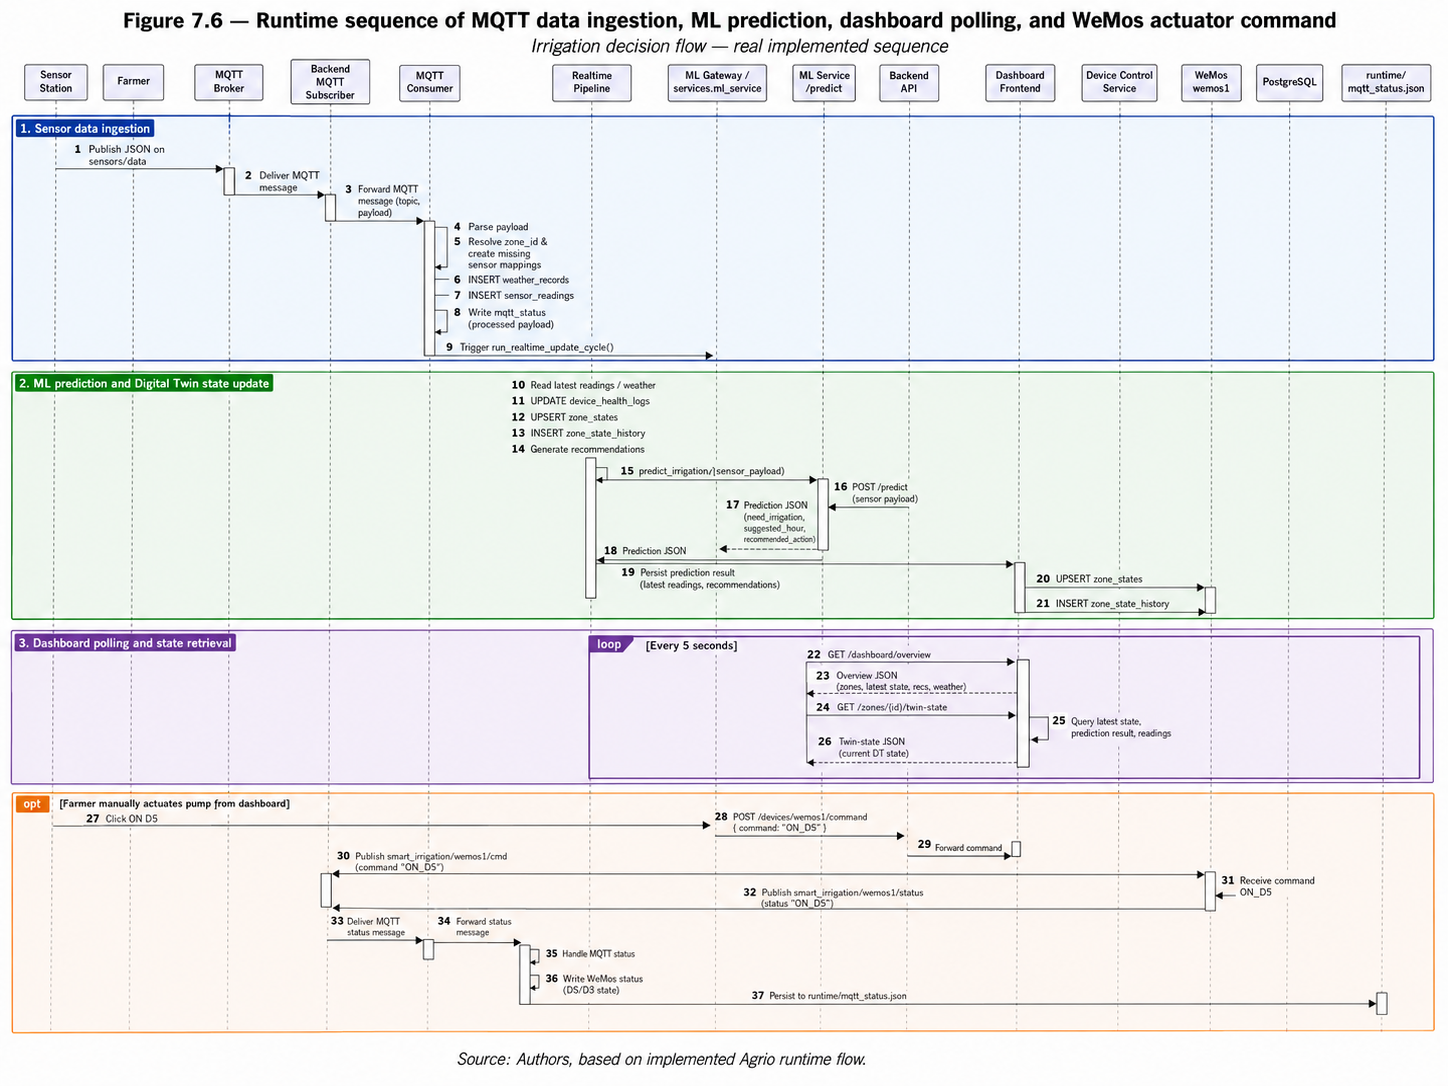
\includegraphics[width=0.9\textwidth,height=0.75\textheight,keepaspectratio]{figures/chapter_07/Figure 7.6 — Runtime sequence of MQTT data ingestion, ML prediction, dashboard polling, and WeMos actuator command.png}
    \caption{Runtime sequence of MQTT data ingestion, ML prediction, dashboard polling, and WeMos actuator command. Source: Authors.}
    \label{fig:7-1-runtime-sequence-of-mqtt-data-ingestion-ml-prediction-dashboard-po}
\end{figure}

\section{Error handling and fallback}

If payload validation fails, the ingestion is marked as ignored or error. If the ML service is unavailable, the system can build a fallback rule-based prediction and store a fallback twin state. This prevents complete workflow failure when the ML service is temporarily unavailable.

\section{Conclusion}

The backend and data ingestion implementation prove that Agrio is not only a frontend demonstration. It contains a real data pipeline from MQTT ingestion to database persistence, Digital Twin synchronization, prediction, recommendation, and control.

\begin{figure}[H]
    \centering
    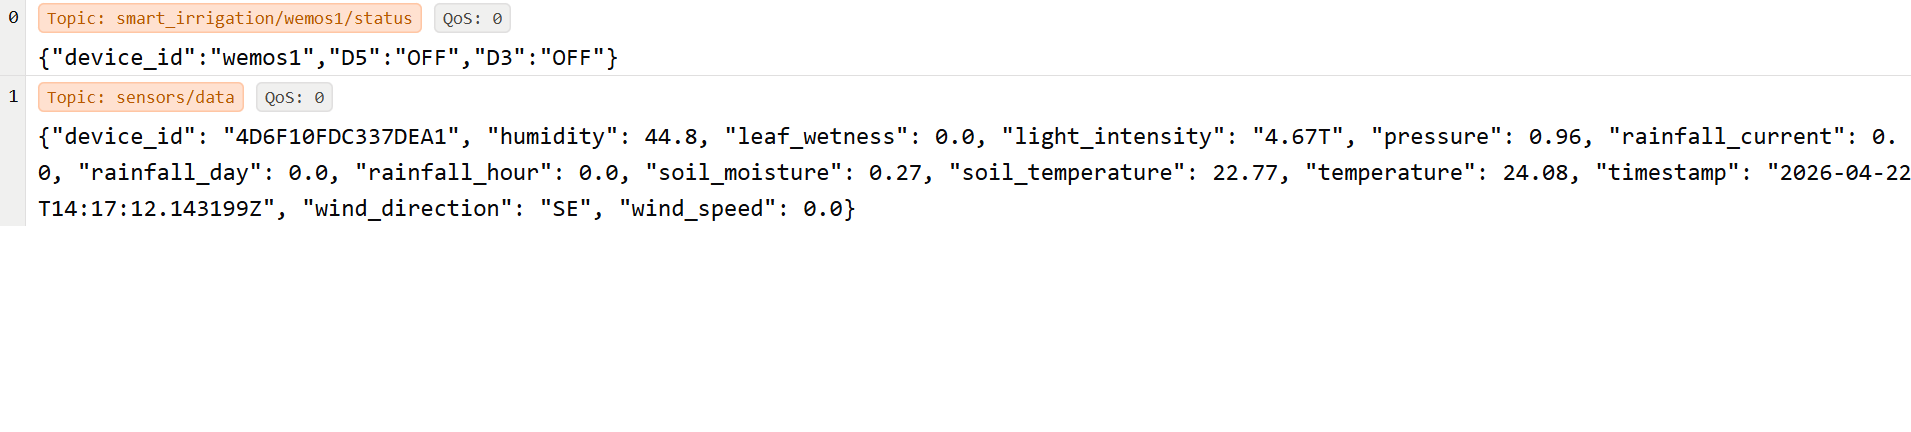
\includegraphics[width=0.9\textwidth,height=0.75\textheight,keepaspectratio]{figures/chapter_07/Figure 7.7 — Live MQTT payloads received through HiveMQ for sensor data and WeMos status.png}
    \caption{Live MQTT payloads received through HiveMQ for sensor data and WeMos status. Source: Authors.}
    \label{fig:7-2-live-mqtt-payloads-received-through-hivemq-for-sensor-data-and-wem}
\end{figure}

\begin{figure}[H]
    \centering
    % \includegraphics[width=0.9\textwidth]{figures/chapter_07/fig_7-3_fastapi-openapi-documentation-exposing-the-re.png}
    \fbox{\parbox{0.85\textwidth}{\centering Insert Figure 7.3 here: FastAPI OpenAPI documentation exposing the REST endpoints of the backend.}}
    \caption{FastAPI OpenAPI documentation exposing the REST endpoints of the backend. Source: Authors.}
    \label{fig:7-3-fastapi-openapi-documentation-exposing-the-rest-endpoints-of-the-b}
\end{figure}

\begin{figure}[H]
    \centering
    % \includegraphics[width=0.9\textwidth]{figures/chapter_07/fig_7-4_postgresql-stored-sensor-readings-persisted-f.png}
    \fbox{\parbox{0.85\textwidth}{\centering Insert Figure 7.4 here: PostgreSQL stored sensor readings persisted from MQTT-originated measurements.}}
    \caption{PostgreSQL stored sensor readings persisted from MQTT-originated measurements. Source: Authors.}
    \label{fig:7-4-postgresql-stored-sensor-readings-persisted-from-mqtt-originated-m}
\end{figure}

\begin{footnotesize}
\setlength{\tabcolsep}{2pt}
\begin{longtable}{@{}>{\raggedright\arraybackslash}p{0.28\textwidth}>{\raggedright\arraybackslash}p{0.28\textwidth}>{\raggedright\arraybackslash}p{0.28\textwidth}@{}}
\caption{Main database groups}\\
\toprule
Group & Tables / examples & Purpose \\
\midrule
\endfirsthead
\toprule
Group & Tables / examples & Purpose \\
\midrule
\endhead
Agricultural structure & users, farms, plots, management\_zones, soil\_profiles, crops & Represent physical organization of the farm and monitored zones \\
Acquisition & sensors, sensor\_readings, weather\_records, device\_health\_logs & Store IoT measurements and device condition \\
Forecasting & forecast\_locations, weather\_forecasts, irrigation\_forecasts & Support weather-aware planning \\
Digital Twin & digital\_twins, zone\_states, zone\_state\_history & Maintain virtual state and historical evolution \\
Prediction/simulation & prediction\_results, twin\_predictions, simulation\_scenarios, simulation\_results & Store ML and what-if outputs \\
Decision/control & recommendations, alerts, irrigation\_events, control\_commands, execution\_feedback & Trace decisions and physical action \\
\bottomrule
\end{longtable}
\end{footnotesize}
